
\mode<presentation>
{
  \usetheme{CambridgeUS}
  \usecolortheme{whale}
  \usecolortheme{lily}

  \setbeamercovered{transparent}
  \usefonttheme[onlymath]{serif}
}

\title[\DisturbancesandSteadyStateErrorShortName] % (optional, use only with long paper titles)
{\course: \DisturbancesandSteadyStateErrorName\license}

\subtitle
{Lecture \DisturbancesandSteadyStateErrorNumber} % (optional)


\begin{document}

\begin{frame}
  \titlepage
\end{frame}

\mode<article>{
\maketitle
\tableofcontents
}


\section{Pre-requisite Material}
This lecture assumes that the reader is familiar with the following material:
\begin{itemize}
\item Lecture \ModelingMechanicalSystemsNumber:~\ModelingMechanicalSystemsName
\item Lecture \SolvingDifferentialEquationsAndStabilityNumber:~\SolvingDifferentialEquationsAndStabilityName
\item Lecture \BlockDiagramsNumber:~\BlockDiagramsName
\end{itemize}

\section{Control for Steady-State Performance Metrics}
In Lectures~\ControlAndStabilityNumber-\PDControlTransientNumber, we were largely focused on control for transient behavior (with a small amount of steady-state behavior discussed as the DC gain). In this lecture through Lecture~\PIDControlDesignNumber, we'll look more in depth at control for steady-state performance, although it should be emphasized that there will always be overlap between the two.

There are two parts to steady-state performance. The first, which is the focus of this lecture, is how a controller is able to reject disturbances, i.e., make the (uncontrollable) disturbance input not matter as much to the output signal. In Lecture~\ReferenceSteadyStateErrorNumber, we'll use some similar concepts and add more to describe how to create controllers that can cause a plant's output signal to better track the desired (reference) input.

\section{The Effect of Disturbances
\label{sec:disteffect}}

A common use for control systems is to reject disturbances. An example would be a control system that implements the cruise control for an automobile. The car of mass $m$ is propelled by its motor, which applies force $f$. This force is something we can control.  The car moves at velocity $\dot{x}$. For convenience, we will define $v=\dot{x}$. There is a drag force due to the wind that we will approximate as a laminar drag term $b\dot{x}=bv$. The road supports the car with contact force $f_{c}$. Finally, there is an external disturbance given by the component of the gravitational force that acts in the $x$ direction whenever there is a hill.  
\begin{frame}{Cruise Control}
\begin{center}
\begin{minipage}{2.1in}
\begin{tikzpicture}[very thick,
sysblock/.style={draw,rectangle,inner sep=6pt,minimum width=1.5cm,minimum height=1.2cm,very thick},
delayblock/.style={draw,rectangle,inner sep=6pt,minimum width=0.5cm,minimum height=1.0cm,very thick},
node/.style={fill,inner sep=0pt,outer sep=0pt},
summer/.style={circle,draw,very thick,inner sep=5pt}]

\draw (3.5,.8) node[rotate=9,above,fill=gray,rectangle,minimum width=2cm, minimum height=0.5cm,rounded corners] (M) {};
\draw (3.4,1.1) node[rotate=9,above,fill=gray,trapezium,trapezium angle=60,minimum width=1.4cm, minimum height=0.5cm,rounded corners] {};
\draw[|->,thin] (M.-90) ++(0,-.45) -- ++(9:1) node[right] {$v=\dot{x}$}; 
\draw (3,.5) node[summer,above,fill=black,draw=white] (W1) {};
\draw (W1) node[circle,fill=gray,inner sep=0pt,outer sep=0pt,minimum height=.1cm] {};
\draw (4,.65) node[summer,above,fill=black,draw=white] (W2) {};
\draw (W2) node[circle,fill=gray,inner sep=0pt,outer sep=0pt,minimum height=.1cm] {};
\draw (1,.3) .. controls +(.11,0) and +(-.5,-.1) .. (3,.5) .. controls +(.5,.1) and +(-.1,-.1) .. (6,1) node[right] {}; 


\end{tikzpicture}\end{minipage}\begin{minipage}{1.7in}
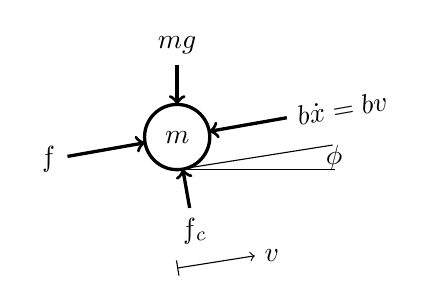
\begin{tikzpicture}[very thick,
sysblock/.style={draw,rectangle,inner sep=6pt,minimum width=1.5cm,minimum height=1.2cm,very thick},
delayblock/.style={draw,rectangle,inner sep=6pt,minimum width=0.5cm,minimum height=1.0cm,very thick},
node/.style={fill,inner sep=0pt,outer sep=0pt},
summer/.style={circle,draw,very thick,inner sep=5pt,outer sep=0pt}]

\draw (0,0) node[summer] (M1) {$m$};

\draw[thin]  (M1.-90) -- ++(2,0);
\draw[thin]  (M1.-90) -- ++(9:2);
\draw (M1.-90) ++(4.5:2) node {$\phi$};
\draw[|->,thin] (M1.-90) ++(0,-1.25) -- ++(9:1) node[right] {$v$}; 
\draw[->] (M1.190) ++(10:-1) node[rotate=10,left] {$f$} -- (M1.190);
\draw[->] (M1.90) ++(0,0.5) node[above] {$mg$} -- ++(0,-0.5);
\draw[->] (M1.-80) ++(-80:0.5) node[rotate=10,below] {$f_{c}$} -- (M1.-80);
\draw[->] (M1.10) ++(10:1) node[rotate=10,right] {$b\dot{x}=bv$} -- (M1.10);

\end{tikzpicture}\end{minipage}
\mode<presentation>{\[
m\ddot{x} = f - b\dot{x} - mg\sin(\phi) 
\]
\[
m\dot{v} +bv = f - f_{d} 
\]}
\end{center}
\end{frame}

In order to use Newton's law, we need to have a non-accelerating reference frame. This means that if we sum the forces in the instantaneous direction of motion, and write
\[
m\ddot{x}(t) = f(t) - b\dot{x}(t) - mg\sin(\phi),
\]
this is correct only if the angle $\phi$ is {\em fixed} (i.e. a hill with a constant slope). (Note that $f_{c}$ is always perpendicular to the direction of motion, and thus does not appear.) However, this equation will be a good approximation if $\phi$ varies {\em slowly}, and since in most roads this is the case, we will use this model to design our control system, even though $\phi$ is not really fixed. 

Let's designate $d(t) = g\sin(\phi)$ to be the component of the gravity force that acts on the car's motion. In addition, let's write this equation in terms of $v=\dot{x}$. The system model is then
\[
m\dot{v}(t) + bv(t) = f(t) - md(t)
\]
Taking the Laplace Transform of both sides, assuming zero initial conditions, 
\[
msV(s)+bV(s) = F(s) - mD(s)
\]
or
\[
V(s) = \frac{1}{ms+b}(F(s) - mD(s))
\]
where $V(s)$ is the Laplace transform of the car's velocity, $F(s)$ is the Laplace transform of the force input under our control, and $D(s)$ is the Laplace Transform of the disturbance due to gravity and a sloped road. Note that this system has two inputs: a controllable one ($F(s)$) and an uncontrollable one ($D(s)$). Thus, we'll need to incorporate a ``sum'' block into our block diagram modeling the plant system, as follows:

%We can create a (simple) block diagram for the car system as follows:
\newpage \begin{frame}{System block diagram}
\begin{center}
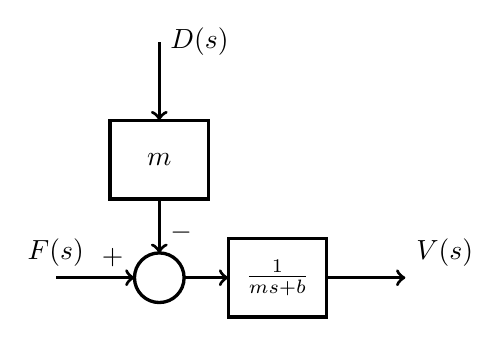
\begin{tikzpicture}[inner sep=0pt,outer sep=0pt,very thick,
sysblock/.style={draw,rectangle,inner sep=2pt,minimum width=1.25cm,minimum height=1.0cm,very thick}]

\draw (0,0) node[draw,circle] (sum) {$\rule{0pt}{18pt}$};
\draw (1.5,0) node[sysblock] (a) {$\frac{1}{ms+b}$};
\draw (0,1.5) node[sysblock] (b) {$m$};

\draw[<-] (sum.180) node[above left=4pt] {$+$} -- ++(-1,0) node[above=4pt] {$F(s)$};
\draw[->] (sum.0) -- (a.180);
\draw[<-] (sum.90) node[above right=4pt] {$-$}  -- (b.-90);
\draw[<-] (b.90) -- ++(0,1)  node[right=4 pt] {$D(s)$};
\draw[->] (a.0) -- ++(1,0) node[above right=4pt] {$V(s)$};

\end{tikzpicture}
\end{center}
%\end{frame}

\mode<article>{Now consider the following questions:}

\begin{enumerate}
\item<2-> Suppose the motor supplies a constant force $f_{m}$ on a flat road. At steady state, what will the car's speed be? 
\item<3-> Suppose the car is at steady state on a flat road, but then drives on an incline with slope $\phi$. By how much will the car slow down?
\end{enumerate}
\end{frame}

To answer the first question, we could find $F(s)$, multiply it by $\frac{1}{ms+b}$, find the inverse Laplace Transform to find $v(t)$, and then find $\lim_{t\rightarrow \infty}v(t)$. A similar process could be done to answer the second question. However, since we are only interested in $\lim_{t\rightarrow \infty}v(t)$, or what is called the {\em final value} of $v(t)$, this is more work than we need to do! For stable systems that have a steady-state response, a much easier alternative is given by the final value theorem.

\section{Final Value Theorem}

The questions listed above require us to determine the steady state response of a system. This is what the output becomes after the transients go to zero.

\begin{frame}{Steady State}
\begin{center}
\begin{tikzpicture}[inner sep=0pt,outer sep=0pt,very thick,
sysblock/.style={draw,rectangle,inner sep=2pt,minimum width=1.5cm,minimum height=1.25cm,very thick}]
\draw (0.6,0) node {\includegraphics[height=1in]{figures/input}};
\draw (4,0) node[sysblock] (sys) {$G(s)$};
\draw (7.9,0) node {\includegraphics[height=1in]{figures/output}};
\draw[<-] (sys.180) -- ++(-0.5,0);
\draw[->] (sys.0) -- ++(0.5,0);

\end{tikzpicture}
\end{center}
\end{frame}

If we know $Y(s)$, can we find the steady state response, $\lim_{t\rightarrow \infty}y(t)$, without having to find the complete inverse Laplace transform? Yes! \textit{As long as that steady-state limit exists.}

Suppose we are given a rational function $Y(s)$, with poles $p_{1}$, $p_{2}$, $\cdots$ $p_{n}$. We can consider some cases:
\begin{itemize}
\item $Y(s)$ has a pole with positive real part: In this case, there will be a term in the partial fraction expansion with amplitude that goes to infinity, and $\lim_{t\rightarrow \infty}y(t)$ will either be infinite or will not exist.
\item $Y(s)$ has a pole on the $j\omega$ axis, excluding $s=0$. In this case, there will be a sine or cosine term. Since $y(t)$ will always contain an oscillatory term, the limit will not exist
\item $Y(s)$ has multiple poles at $s=0$. This would correspond to a $t$, $t^{2}$, or other polynomial term, and the limit would be infinite, if it existed.
\item $Y(s)$ has only poles either with a negative real part or a single pole at $s=0$. In this case, the terms decay either to zero or a constant, and $\lim_{t\rightarrow \infty}y(t)$ will exist.
\end{itemize}
Thus, our first conclusion is that the steady state value exists and is finite only if all the poles either have a negative real part, or there is a single pole at $s=0$.

Now, suppose $Y(s)$ has poles in the left half plane and a pole at $s=0$, so that
\[
Y(s) = \frac{A}{s} + \frac{B}{s-p_{1}} + \frac{C}{s-p_{2}} + \cdots
\]
Using the residue formula for partial fraction expansion, we can find
\[
A = \left.sY(s)\right|_{s=0}
\]
The inverse Laplace transform would be
\[
y(t) = A + Be^{p_{1}t} + Ce^{p_{2}t} + \cdots
\]
Since $Y(s)$ has all poles in the LHP (besides the one at $s=0$), all of the other poles $p_i$ have negative real part, all the terms with exponentials will decay to zero. Thus
\[
\lim_{t\rightarrow\infty} y(t) = A
\]
On the other hand, if $Y(s)$ had no pole at $s=0$, $\lim_{t\rightarrow\infty}y(t)=0$, but we would also have $\left.sY(s)\right|_{s=0}=0$. Our conclusions can be summarized in the following result
\begin{frame}
\begin{theorem}
Given the signal $Y(s)$ such that $sY(s)$ has all poles with negative real part. Then the inverse Laplace transform $y(t)$ satisfies
\[
\boxed{\lim_{t\rightarrow\infty} y(t) = \lim_{s\rightarrow 0}sY(s)}
\]
\end{theorem}
\end{frame}

\section{Disturbance Analysis}

Let's apply the final value theorem to answer the questions given near the end of Section~\ref{sec:disteffect}. 
\begin{enumerate}
\item Suppose the motor supplies a constant force $f$ on a flat road. At steady state, what will the car's speed be? In this case, there is no disturbance, so
\[
V(s) = \frac{1}{ms+b}F(s).
\]
The force input is constant, so $F(s) = \frac{f_{m}}{s}$, and
\[
V(s) = \frac{1}{ms+b}\frac{f_{m}}{s}.
\]
For the final value theorem, we need to calculate 
\[
sV(s) = s\frac{1}{ms+b}\frac{f_{m}}{s} = \frac{f_{m}}{ms+b}
\]
Stability check: the signal $sV(s)$ has a pole at $-b/m$. Since both $m$ and $b$ are positive, we can verify that $sV(s)$ has its single pole with negative real part, and the final value theorem can be applied. Thus
\begin{align*}
\lim_{t\rightarrow \infty} v(t) &= \lim_{s\rightarrow 0} sV(s)\\
 &= \lim_{s\rightarrow 0}\frac{f_{m}}{ms+b} \\
 & = \frac{f_{m}}{b}.
\end{align*}
\item Suppose the car is at steady state on a flat road, but then drives on an incline with slope $\phi$. By how much will the car slow down? In this case, the car's velocity is impacted by both the motor and the disturbance
\begin{frame}
\[
V(s) = \frac{1}{ms+b}F(s) - \frac{m}{ms+b}D(s)
\]
\end{frame}
Note that the velocity will be the sum of the two terms - the first due to the motor force $F(s)$, the second due to the force caused by gravity and the hill ($mD(s)$). The amount that the car slows down due to the disturbance is then the steady state value of the second term. Define
\[
V_{d}(s) = \frac{m}{ms+b}D(s),
\]
i.e., this second term. We wish to find $\lim_{t\rightarrow \infty} v_{d}(t)$. From the problem statement, $d(t)$ is a step, with magnitude $g\sin(\phi)$. Thus $D(s) = \frac{g\sin(\phi)}{s}$, and 
\begin{align*}
sV_{d}(s) &= s \frac{m}{ms+b}\frac{g\sin(\phi)}{s} \\
&= \frac{mg\sin(\phi)}{ms+b}.
\end{align*}
Stability check: again, the pole $-b/m$ has negative real part, so the final value theorem applies. We calculate that the amount of slowdown due to the hill (in steady-state) $v_d(t)$ is therefore
\begin{align*}
\lim_{t\rightarrow\infty}v_{d}(t) &= \lim_{s \rightarrow 0}  \frac{mg\sin(\phi)}{ms+b} \\
&= \frac{mg\sin(\phi)}{b} 
\end{align*}
\end{enumerate}

A common use of a feedback control system is to reduce the effect of disturbances. Suppose we apply a feedback control that measures the velocity of the car, and changes the applied force in proportion to the error between a desired speed set-point $v_{set}$ and the measured speed. This feedback control system can be represented by the following block diagram.

\begin{frame}
\begin{center}
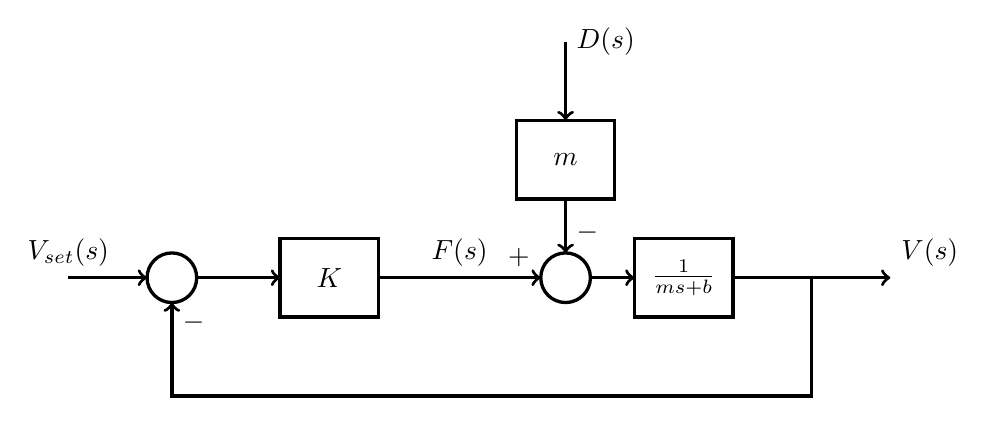
\begin{tikzpicture}[inner sep=0pt,outer sep=0pt,very thick,
sysblock/.style={draw,rectangle,inner sep=2pt,minimum width=1.25cm,minimum height=1.0cm,very thick}]

\draw (-5,0) node[draw,circle] (sum2) {$\rule{0pt}{18pt}$};
\draw (-3,0) node[sysblock] (C) {$K$};
\draw (0,0) node[draw,circle] (sum) {$\rule{0pt}{18pt}$};
\draw (1.5,0) node[sysblock] (a) {$\frac{1}{ms+b}$};
\draw (0,1.5) node[sysblock] (b) {$m$};

\draw[<-] (sum2.180) -- ++(-1,0) node[above=4pt] {$V_{set}(s)$};
\draw[->] (sum2.0) -- (C.180);
\draw[->] (C.0) -- node[above=4pt] {$F(s)$} (sum.180) node[above left=4pt] {$+$};
\draw[->] (sum.0) -- (a.180);
\draw[<-] (sum.90) node[above right=4pt] {$-$}  -- (b.-90);
\draw[<-] (b.90) -- ++(0,1)  node[right=4 pt] {$D(s)$};
\draw[->] (a.0) -- ++(2,0) node[above right=4pt] {$V(s)$};
\draw[->] (a.0) ++(1,0) -- ++(0,-1.5) -| (sum2.-90) node[below right=4pt] {$-$};

\end{tikzpicture}
\end{center}
%\end{frame}

\mode<article>{Using block diagram simplification rules, we get the following formula for $V(s)$:}
\visible<2->{
\[
V(s) = \frac{K}{ms + b + K}V_{set}(s) - \frac{m}{ms+b+K}D(s)
\]}
\end{frame}
When the car is on a level surface, (no disturbances) the speed will be determined by the first term. The change in speed due to a slope will again be due to the second term
\[
V_{d}(s) = \frac{m}{ms+b+K}D(s).
\]
If $d(t) = g\sin(\phi)u(t)$, then
\[
sV_{d}(s) = s\frac{m}{ms+b+K}\frac{g\sin(\phi)}{s} = \frac{mg\sin(\phi)}{ms+b+K}
\]
If we pick $K>0$ so that $b+K>0$, then $sV_{d}(s)$ has a pole with negative real part, and thus we can use the final value theorem.
\begin{align*}
\lim_{t\rightarrow\infty}v_{d}(t) &= \lim_{s\rightarrow 0} sV(s) \\
&= \lim_{s\rightarrow 0} \frac{mg\sin(\phi)}{ms+b+K} \\
 & = \frac{mg\sin(\phi)}{b+K}
\end{align*}
Note that since $K>0$, the change in velocity has been reduced from $ \frac{mg\sin(\phi)}{b}$ in the open loop case to  $\frac{mg\sin(\phi)}{b+K}$

%\section{Application Example}
%
%\noindent In Lecture \HigherOrderResponseNumber \ we derived the relationship between the wind speed \(u\) and the rotational speed of a wind turbine \(\omega\): 
%\begin{equation*}
%\frac{\omega(s)}{u(s)} = \frac{0.54435(s^2+0.09341s+6.511)}{(s+0.2867)(s^2+0.2996s+6.477)} = G_1(s)
%\end{equation*}
%
%Since wind speed is an uncontrollable input to a wind turbine, it is actually a disturbance signal, albeit a very important one. Wind turbines also have several control inputs, which enable a control engineer to control the turbine's operation. One of these control input is the blade pitch angle, normally represented as \(\beta\), and pictured in Figure~\ref{fig:turbine}.
%
%\begin{figure}
%\begin{center}
%	\includegraphics[width=3in]{figures/Figure1.png}
%	\caption{Wind turbine with blade pitch angle rotational degree of freedom shown. \small{Obtained from \url{http://usuaris.tinet.cat/zefir/pitch.htm} on 8/30/15.}}
%	\label{fig:turbine}
%\end{center}
%\end{figure}
%
%The transfer from the control input \(\beta\) to the rotational speed \(\omega\) is
%
%\begin{equation*}
%\frac{\omega(s)}{\beta(s)} = \frac{-21.201(s^2+0.04283s+6.509)}{(s+0.2867)(s^2+0.2996s+6.477)} = G_2(s)
%\end{equation*}
%
%\noindent The wind turbine plant can therefore be represented as a sum of the two inputs (control and disturbance) multiplied by their respective transfer functions, or
%\begin{equation*}
%\omega(s) = G_1(s)u(s)+G_2(s)\beta(s)
%\end{equation*}
%as shown in Figure~\ref{fig:diagram}. Note that the denominators of \(G_1(s)\) and \(G_2(s)\) are equal; this is not a coincidence, but rather an inherent property of the wind turbine plant.\\
%
%\begin{figure}
%	\begin{center}
%	\includegraphics[width=2.5in]{figures/Turbine.png}
%	\caption{Wind turbine plant shown with disturbance input \(u\) (wind speed) and control input \(\beta\) (blade pitch angle).}
%	\label{fig:diagram}
%\end{center}
%\end{figure}
%
%
%\noindent \textbf{Thought Experiment:} Using your intuition about the wind turbine system, do you expect the wind turbine plant to be BIBO stable or not with respect to
%
%\begin{enumerate}[(a)]
%	\item The disturbance input \(u\)?
%	\item The control input \(\beta\)?
%\end{enumerate}
%
%\noindent \textbf{Intuition Argument:} If we imagine a bounded wind speed input, it's hard to imagine an unbounded rotor speed (though both may get very high). Similarly, changing the blade pitch angle seems unlikely to drive the rotor speed to infinity.\\
%
%\noindent \textbf{Mathematical Argument:}  Of course, we can check our answers using control theory by looking at the pole locations, which in fact we already did in Lecture \HigherOrderResponseNumber. All three plant poles 
%\begin{equation*}
%s_i = \{-0.150 \pm j2.54, -0.287\}
%\end{equation*}
%are in the open left-half plane (real part strictly less than zero), which proves our intuition correct: the wind turbine plant is BIBO stable.
%
%


\section{Lecture Highlights}
The primary takeaways from this article include
\begin{enumerate}
\setlength{\itemsep}{5pt}
\setlength{\parskip}{0pt}
\setlength{\parsep}{0pt}
\item Disturbances are system inputs that cannot be controlled. 
\item A system can have multiple inputs. In the case noted in this article, we can analyze the impacts of the control input and disturbance input separately by temporarily setting the other input equal to zero. In the car example, we have $V(s) = G_1(s)F(s) + G_2(s)D(s)$. 
\item The Final Value Theorem (FVT) allows us to determine the steady-state value of a signal $y(t)$ without having to compute $y(t)$ via differential equation techniques \textit{if a steady-state value exists}. Before applying the FVT, make sure to check that the Laplace domain signal $Y(s)$ has all poles in the left half plane, with the exception of one allowable pole at $s=0$.
\end{enumerate}


\section{Quiz Yourself}

\subsection{Questions}


\begin{enumerate}
\setlength{\itemsep}{5pt}
\setlength{\parskip}{0pt}
\setlength{\parsep}{0pt}
\item For the following system, find the steady state effect on the output for a ramp disturbance ($D(s)$).
\begin{center}
\input{quizfigures/system2.tex}
\end{center}
\item A feedback control system is subject to disturbances at the actuator input, as shown in the following block diagram. 
\begin{center}
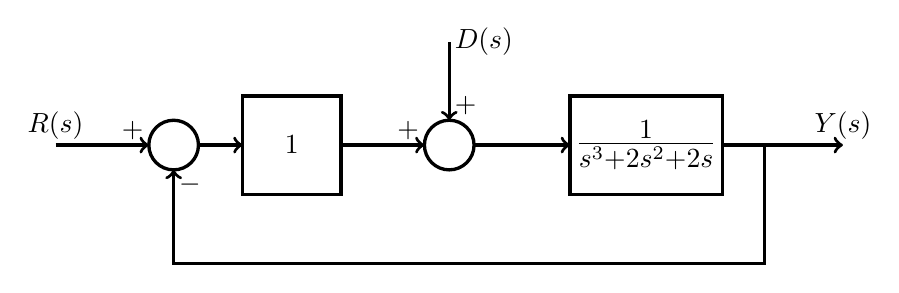
\begin{tikzpicture}[scale=1,inner sep=0pt,outer sep=0pt,very thick,
sysblock/.style={draw,rectangle,inner sep=2pt,minimum width=1.25cm,minimum height=1.25cm,very thick}]
\draw (2,0) node[draw,circle] (sum1) {$\rule{0pt}{18pt}$};
\draw (3.5,0) node[sysblock] (Kp) {$1$};
\draw (5.5,0) node[draw,circle] (sum2) {$\rule{0pt}{18pt}$};
\draw (8,0) node[sysblock] (G) {\Large $\frac{1}{s^{3}+2s^{2}+2s}$};
\draw[->] (.5,0) node[above=2pt] {$R(s)$} -- (sum1.180) node[above left=2pt] {$+$};
\draw[<-] (sum2.90) node[above right=2pt] {$+$} -- ++(0,1) node[right=2pt] {$D(s)$};
\draw[->] (sum1.0) --  (Kp);
\draw[->] (Kp) -- (sum2.180) node[above left=2pt] {$+$};
\draw[->] (sum2) -- (G);
\draw[->] (G) -- ++(2.5,0) node[above=2pt] {$Y(s)$};
\draw[->] (G) ++(1.5,0) -- ++(0,-1.5) -| (sum1.-90) node[below right=2pt] {$-$};
\end{tikzpicture}
\end{center}
If the reference command is $r(t)=0$, what is the steady state output if the disturbance is
\begin{enumerate}
\item A unit step $d(t)=u(t)$
\item A unit ramp $d(t)=tu(t)$.
\end{enumerate}
\end{enumerate}


\subsection{Solutions}
\begin{enumerate}
\setlength{\itemsep}{5pt}
\setlength{\parskip}{0pt}
\setlength{\parsep}{0pt}
\item \rule{0pt}{12pt}\\
\begin{center}
\includegraphics[width=5in]{quizfigures/1soln}\\
\end{center}
\item \rule{0pt}{12pt}\\
\includegraphics[width=5in]{quizfigures/2soln}\\
\end{enumerate}

\section{Resources}

\subsection{Books}


\begin{itemize}
\item Norman S. Nise, {\em Control Systems Engineering}, Wiley
\begin{itemize}
\item 7th edition: Section 7.5
\end{itemize}
\item Richard C. Dorf and Robert H. Bishop, {\em Modern Control Systems}, Pearson
\begin{itemize}
\item 13th edition: Section 4.4
\end{itemize}
\item Gene F. Franklin, J. David Powell and Abbas Emami-Naeini,  {\em Feedback Control of Dynamic Systems}, Pearson
\begin{itemize}
\item 6th and 7th edition: Section 4.2.2
\end{itemize}
\end{itemize}


\subsection{Web resources}

If you find any useful web resources, please contact your instructor.


\end{document}
